\documentclass[electronic]{kthesis}

%%%%%%%%%%%%%%%%%
%%%% PACKAGES %%%
%%%%%%%%%%%%%%%%%
\usepackage[utf8x]{inputenc}
\usepackage[swedish,english]{babel}
\usepackage{enumerate}  % for capital latin numbers in the list of papers
\usepackage{caption}   % to align the table caption to the right/left
\usepackage{lscape}
\usepackage{hyperref}  %for references
\usepackage{amsmath,mathrsfs}
\usepackage{amssymb}  % assumes amsmath package installed
\usepackage{epstopdf}
\usepackage{subfig}
\usepackage{cite}
\usepackage{hyperref}
\usepackage{graphicx}
\usepackage{bm}	%Command \bm{make bold}
\usepackage{algorithm}
\usepackage{algpseudocode}
\usepackage{algpascal}
\usepackage{multicol}
\usepackage[x11names]{xcolor}
\usepackage{lipsum}

\usepackage{tikz}
\usetikzlibrary{tikzmark,calc,decorations.pathreplacing}
\newcommand{\Depth}{2}
\newcommand{\Height}{2}
\newcommand{\Width}{2}

\renewcommand{\labelitemi}{\textcolor{IndianRed3}{\bfseries\textbullet}}


%%%%%%%%%%%%%%%%%%%%%%%%%%%%%%%%%%%%%%%
%%%%%%%%% Document starts here %%%%%%%%
%%%%%%%%%%%%%%%%%%%%%%%%%%%%%%%%%%%%%%%
\begin{document}
	
	%%%%%%%%%%%%%%%%%%%%%%%%%%%%%%%%%%%%%%%%%%
	%%%%%% First and second pages %%%%%%%%%%%%
	%%%%%%%%%%%%%%%%%%%%%%%%%%%%%%%%%%%%%%%%%%
	\title{ Thesis Title }
	\subtitle{\textbf{sub-title}}
	\author{Marcus Klasson}
	\date{date}
	\thesistype{Doctoral Thesis}
	\imprint{Stockholm, Sweden, 2020}
	\examen{Teknologie doktorexamen i elektroteknik}
	\disputationsdatum{fredagen den 18 januari 2020 klockan 14.00}
	\disputationslokal{Sal F3, Lindstedtsvägen 26, Kungliga Tekniska H\"{o}gskolan, Stockholm}
	\publisher{Universitetsservice US AB}
	\address{KTH Royal Institute of Technology \\School of Electrical Engineering and Computer Science\\ Division of Fusion Plasma Physics \\ SE-10044 Stockholm\\ Sweden}
	\isbn{ISBN 100-}
	%\issn{ISSN XXX} % No longer used at KTH
	\trita{TRITA-EECS-AVL-2020:4}
	\kthlogo{KTHLogo}
	
	% Create title page using info above
	\maketitle
	
	\frontmatter % Pages i, ii, iii, iv, v etc.
	%%%%%%%%%%%%%%%%%%%%%%%%%%%%%%%%%%%
	%%%%%%%%%%% ABSTRACT %%%%%%%%%%%%%%
	%%%%%%%%%%%%%%%%%%%%%%%%%%%%%%%%%%%
	\begin{abstract}

\noindent In recent years, computer vision-based assistive technologies have enabled visually impaired people to use automatic visual recognition on their mobile phones. 
These systems should be capable of recognizing objects on fine-grained levels to provide the user with accurate predictions. Additionally, the user should have the option to update the system continuously to recognize new objects of interest. 
However, there are several challenges that need to be tackled to enable such features with assistive vision systems in real and highly-varying environments. 
For instance, fine-grained image recognition usually requires large amounts of labeled data to be robust. %, and
Moreover, image classifiers struggle with retaining performance of previously learned abilities when they are adapted %adapting 
to new tasks. 
This thesis is divided into two parts where we address these challenges. 
First, we focus on the application of using assistive vision systems for grocery shopping, where items are naturally structured based on fine-grained details.  
We demonstrate how image classifiers can be trained with a combination of natural images and web-scraped information about the groceries to obtain more accurate classification performance compared to only using natural images for training. 
Thereafter, we bring forward a new approach for continual learning called replay scheduling, where we select which tasks to replay at different times to improve memory retention. 
Furthermore, we propose a novel framework for learning replay scheduling policies that can generalize to new continual learning scenarios for mitigating the catastrophic forgetting effect in image classifiers. 
This thesis provides insights on practical challenges that need to be addressed to enhance the usefulness of computer vision for assisting the visually impaired in real-world scenarios. 

\begin{comment}
\noindent In recent years, computer vision-based assistive technologies have enabled visually impaired people to use automatic visual recognition on their mobile phones. 
These systems should be capable of recognizing objects on fine-grained levels to provide the user with accurate predictions. Additionally, the user should have the option to update the system continuously to recognize new objects of interest.  %Moreover, a valuable feature would be if they could be updated to recognize new object classes. 
However, there are several challenges that need to be tackled to enable such features with assistive vision systems in real and highly-varying environments. 
For instance, fine-grained image recognition usually requires large amounts of labeled data to be robust, and image classifiers struggle with retaining performance of previously learned abilities when adapting to new tasks. 
This thesis is divided into two parts where we address these challenges. 
First, we focus on the application of using assistive vision devices for grocery shopping where items are naturally structured based on fine-grained details.  %grocery shopping with an assistive vision device where items are naturally structured based on fine-grained details. 
We demonstrate how image classifiers can be trained with a combination of natural images and web-scraped information about the groceries to obtain more accurate classification performance compared to only using natural images for training. %To reduce the need for exhaustive data collection in grocery stores, we show how image classifiers can be trained with a combination of real images and web-scraped information about the groceries to obtain more accurate classification performance.
Secondly, we bring forward a new approach for continual learning called replay scheduling where we select which tasks to replay at different times to improve memory retention. 
Furthermore, we propose a novel framework for learning replay scheduling policies that can generalize to new continual learning scenarios for mitigating the catastrophic forgetting effect in image classifiers. 
This %To summarize, this 
thesis provides insights on practical challenges that need to be addressed to enhance the usefulness of computer vision for assisting the visually impaired in real-world scenarios. 
\end{comment}



%To address these challenges, 

%Problems with fine-grained image recognition is that it requires large amounts of training data for being robust in real environments with high-variations. 

%The problem with updating the object recognizer continuously is that the recognizer typically suffers from catastrophic forgetting, such that it is hard to guarantee that the recognizer will accurately recognize previously learned objects after learning new ones. 

%This thesis has been divided into two parts targeting these challenges. For fine-grained recognition, we focus on the application of grocery shopping with an assistive vision device. To reduce the need for exhaustive data collection in grocery stores, we show how image classifiers can be trained with a combination of real images and web-scraped information about the groceries to obtain more accurate classification performance. 

%In continual learning, we bring forward a new approach called replay scheduling where we select which tasks to replay at different times. Moreover, we propose a framework for learning replay scheduling policies that can generalize to new continual learning scenarios for mitigating catastrophic forgetting. 


%This thesis provides approaches motivated from real-world applications as well as insights towards automatic visual recognition to assist the visually impaired. 

%To tackle the challenges with fine-grained image recognition, we propose combining learning from web information to reduce the need for collecting real-world images. We have collected a dataset of grocery items in addition to web-scraped information of the items and suggest a method based on multi-view representation learning that enhances the classification performance when combing learning fro real images and web information over learning from only real images. 

%To tackle the catastrohic forgetting, we propose a novel approach called repla yscheduling for mititgating catastrophic forgetting where we select which old tasks to rehearse on at differetn times. We show that repla yscheduling is important in continual learning settings as well as propose a method to enable more efficient scheduling policies that can generalzie to new scenarios without added training cost. 

%Why is this work imporatnt for assistive vision?


%These systems should be capable of recognizing objects that are important for the user on a fine-grained level. To this end, we have focused on the particular application of classifying food items which can be challenging for blind/low-vision people since visual information is often required for distinguishing between similar items. In Paper A, we present a challenging image dataset of groceries taken in grocery stores where each item is hierarchically labeled to capture the fine-grained structure of the various items. Furthermore, we demonstrate in Paper B how more easily accessible information about the items, such as web-scraped images and text descriptions, can be utilized for enhancing the classification performance of groceries compared to only using the real-world images for training. 

%A valuable feature of assistive vision systems is the capability of adapting to new object classes. The main challenge here is to avoid catastrophically forgetting previously learned knowledge when the classifier is updated with new classes. In Paper C, we propose a new continual learning setting for replay-based methods that aligns well with real-world needs where constraints are placed on processing time rather than the storage capacity of old samples. 
%Replay methods mitigate this problem efficiently by mixing previous data samples from a limited memory buffer with the training samples of the new classes during learning. In Paper C, we propose a new continual learning setting that is close to real-world needs where constraints are placed on processing time rather than the storage capacity of old samples. 
%We then study the timing of replaying certain tasks and show that learning replay schedules over which tasks to replay can be critical for the final classification performance in our proposed setting. Finally, in Paper D, we present a method based on reinforcement learning for learning a policy for selecting which tasks to replay at different times. The benefit of our learned replay scheduling policy is that it can be applied to any new continual learning scenario for mitigating catastrophic forgetting in a classifier without additional computational cost. 

%To conclude, I will discuss some potential future directions for the development of the next generation of computer vision-based assistive technologies. 
	
\begin{comment}
\noindent In recent years, computer vision-based assistive systems have enabled visually impaired people to use automatic object recognition on their mobile phones. 
These systems should be capable of recognizing objects that are important for the user on a fine-grained level. 
To this end, we have focused on the particular application of classifying food items which can be challenging for blind/low-vision people since visual information is often required for distinguishing between similar items. 
In Paper A, we present a challenging image dataset of groceries taken in grocery stores where each item is hierarchically labeled to capture the fine-grained structure of the various items. 
Furthermore, we demonstrate in Paper B how more easily accessible information about the items, such as web-scraped images and text descriptions, can be utilized for enhancing the classification performance of groceries compared to only using the real-world images for training. 

A valuable feature of assistive vision systems is the capability of adapting to new object classes. 
The main challenge here is to avoid catastrophically forgetting previously learned knowledge when the classifier is updated with new classes. 
In Paper C, we propose a new continual learning setting for replay-based methods that aligns well with real-world needs where constraints are placed on processing time rather than the storage capacity of old samples. 
%Replay methods mitigate this problem efficiently by mixing previous data samples from a limited memory buffer with the training samples of the new classes during learning. In Paper C, we propose a new continual learning setting that is close to real-world needs where constraints are placed on processing time rather than the storage capacity of old samples. 
We then study the timing of replaying certain tasks and show that learning replay schedules over which tasks to replay can be critical for the final classification performance in our proposed setting. 
Finally, in Paper D, we present a method based on reinforcement learning for learning a policy for selecting which tasks to replay at different times. The benefit of our learned replay scheduling policy is that it can be applied to any new continual learning scenario for mitigating catastrophic forgetting in a classifier without additional computational cost. 

To conclude, I will discuss some potential future directions for the development of the next generation of computer vision-based assistive technologies. 
\end{comment}



%which have been mostly ignored in the literature, can have a high influence on the final classification performance. We then propose a new continual learning setting where scheduling over which tasks to replay becomes important 


%, where replay methods common approach to mitigate this problem is by using replay methods which involve mixing a small set of previous data samples with the samples from the new classes to learn during training.

%In the second part of my work, I have focused on continually learning new object classes where the main challenge is to avoid forgetting previously learned knowledge when the classifier is updated with new classes. 

%A common approach to mitigate this problem is by using replay methods which involve mixing a small set of previous data samples with the samples from the new classes to learn during training. However, current replay methods have ignored the time of when to replay certain tasks, which would be essential for fast adaptation in settings where constraints are set on training time rather than storage capacity of old samples. In Paper C, we show that learning the time to learn which tasks to replay can be critical for the CL performance in this setting. 

%In Paper D, we present a method for learning a policy for selecting which tasks to replay at different times with reinforcement learning.      

%Finally, I will discuss future directions and potential research questions for the development of the next generation of computer vision-based assistive technologies. 


\bigskip \bigskip







%50\%:
%The recent advances in computer vision have made it possible to develop vision-based assistive devices to aid visually impaired people with object recognition in different environments. A particular application where assistive vision would be useful is to help the visually impaired with fine-grained classification of food items since visual information is often required to distinguish between similar items. 
%Enabling image classification models to work in this setting requires collecting large amounts of images of food items which is an expensive process in several ways. In the first part of my work, I have shown how more easily accessible information about food items, such as web-scraped images and text descriptions, can be used for enhancing the classification performance of groceries compared to training using natural images only. 

%A valuable feature of assistive vision devices is the capability of adapting to new object classes. The key challenge is to avoid overwriting previous knowledge when the model is updated with new classes, which is called catastrophic forgetting. In the second part of my work, I aim to mitigate this problem using replay methods, which involve mixing previous data samples with incoming samples from new classes during training. 

%Finally, I will discuss a future third part consisting of approaches for scaling replay methods to larger datasets and how to deploy our models in mobile devices.
		
\end{abstract}
	
\bigskip \bigskip \bigskip \bigskip \bigskip
	
%\setlength{\leftskip}{0.3 cm} \textbf {Keywords:} Visual Recognition, Fine-grained Classification, Continual Learning, Visually Impaired People, Assistive Technologies

	
	%%%%%%%%%%%%%%%%%%%%%%%%%%%%%%%%%%%%%%%%
	%%%%%%%% SWEDISH ABSTRACT %%%%%%%%%%%%%%
	%%%%%%%%%%%%%%%%%%%%%%%%%%%%%%%%%%%%%%%%
	\newpage
	\selectlanguage{swedish}
\begin{abstract}
\noindent hej
\end{abstract}
\selectlanguage{english}

	
	%%%%%%%%%%%%%%%%%%%%%%%%%%%%%%%%%%%%%%%
	%%%%%%% List of papers %%%%%%%%%%%%%%%%
	%%%%%%%%%%%%%%%%%%%%%%%%%%%%%%%%%%%%%%%
	%*******************************************************************************
%*********************************** List of Papers ****************************
%*******************************************************************************

\chapter{List of Papers}
\label{chap:list_of_papers}

%\let\thefootnote\relax\footnote{Paper I and III are published under license in \textit{Journal of X}}
\begin{enumerate}[A]
	\item \textbf{\textit{A Hierarchical Grocery Store Image Dataset with Visual and Semantic Labels}} \\
	\textbf{Marcus Klasson}, Cheng Zhang, Hedvig Kjellström \\
	In \textit{IEEE Winter Conference on Applications of Computer Vision (2019)}
\end{enumerate}

\begin{enumerate}[B]
	\item \textbf{\textit{Using Variational Multi-view Learning for Classification of Grocery Items}} \\
	\textbf{Marcus Klasson}, Cheng Zhang, Hedvig Kjellström \\
	In \textit{Patterns, Volume 1(8) (2020)}
\end{enumerate}

\begin{enumerate}[C]
	\item \textbf{\textit{Learn the Time to Learn: Replay Scheduling for Continual Learning}} \\
	\textbf{Marcus Klasson}, Hedvig Kjellström, Cheng Zhang \\
	\textit{Under submission}
\end{enumerate}

\begin{enumerate}[D]
	\item \textbf{\textit{Meta Policy Learning for Replay Scheduling in Continual Learning}} \\
	\textbf{Marcus Klasson}, Hedvig Kjellström, Cheng Zhang \\
	\textit{Under preparation}
\end{enumerate}



\begin{comment}
%%%%%%%%%%%%%%%%%%%%%%%% Papers NOT included in THESIS
Other contributions by the author not included in the thesis.
\begin{enumerate}[I]
	\setcounter{enumi}{1}
	\item \textbf{\textit{Title of paper}} \\
	\textbf{First author}, Second author \\
	\textit{Journal (year)}
\end{enumerate}
\end{comment}


	%%%%%%%%%%%%%%%%%%%%%%%%%%%%%%%%%%%%%%%
	%%%%%%%% ACKNOWLEDGMENT %%%%%%%%%%%%%%%
	%%%%%%%%%%%%%%%%%%%%%%%%%%%%%%%%%%%%%%%
	%*******************************************************************************
%*********************************** Acknowledgements **************************
%*******************************************************************************

\chapter{Acknowledgements}
\label{chap:acknowledgements}

\noindent hej
	
	%%%%%%%%%%%%%%%%%%%%%%%%%%%%%%%%
	%%%%%%%% ACRONYMS %%%%%%%%%%%%%%
	%%%%%%%%%%%%%%%%%%%%%%%%%%%%%%%%
	%*******************************************************************************
%*********************************** Acronyms **********************************
%*******************************************************************************

\chapter{Acronyms}
\label{chap:acronyms}

List of commonly used acronyms: \\

\begin{tabular}{llll}
	\textbf{AE}		&	Acronym examples \\
	\textbf{CL}		& 	Continual Learning \\
	\textbf{ML}		& 	Machine Learning \\
	\textbf{RL}		& 	Reinforcement Learning \\
	\textbf{VAE}		&	Variational Autoencoder \\
	
\end{tabular}
	
	%\input{Content/Dedication}\clearpage
	
	\mainmatter % Pages 1, 2, 3...
	%%%%%%%%%%%%%%%%%%%%%%%%%%%%%%%%%%%%%%
	%%%%%% TABLE OF CONTENTS %%%%%%%%%%%%%
	%%%%%%%%%%%%%%%%%%%%%%%%%%%%%%%%%%%%%%
	\tableofcontents
	
	%%%%%%%%%%%%%%%%%%%%%%%%%%%%%%%%%%%%%%%%%%%%%%%%%%%%%%
	%%%%%%%%%%%%% CHAPTER 1: INTRODUCTION %%%%%%%%%%%%%%%%
	%%%%%%%%%%%%%%%%%%%%%%%%%%%%%%%%%%%%%%%%%%%%%%%%%%%%%%
	\chapter{Energy needs - an introduction}
	\label{Intro}
	Here is an example for referencing figure \ref{EnergySources}. Example of citing \cite{BP2019} and \cite{Chen2016}.
	%%%%%%%%%%%%%% Figure: Energy sources
	\begin{figure}[h]
		\centering
		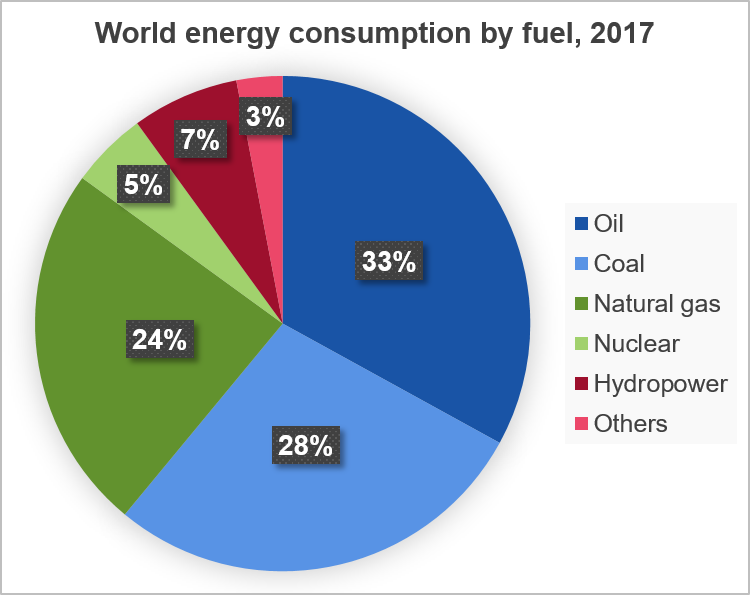
\includegraphics[scale=0.6]{Figs/Ch1_EnergySources.png}
		\caption{The world's energy consumption by fuel in 2017. }
		\label{EnergySources}
	\end{figure}
	
	%%%%%%%%%%%%%%%%%%%%%%%%%%%%%%%%%%%%%%%%
	\section{Section}
	Example of a table
	%%%%%%%%%%%%%%%%%%%%%%%%%%%%%%%% Table: Tokamaks
	\begin{table}[t!]
		\centering
		\caption{List of experimental tokamaks worldwide. Note: ITER is currently under construction and the first plasma is predicted for 2025-2028.}
		\begin{tabular}{ccccc}
			\hline
			\textbf{Name} & \textbf{Location} & \textbf{B-field} & \textbf{Major/minor radius}  \\
			\hline
			JET     & England      & 4.0 T & 3.0 m / 1.3 m \\
			ITER    & France       & 5.3 T & 6.2 m / 2.0 m \\
			AUG		& Germany      & 3.1 T & 1.7 m / 0.7 m \\
			WEST	& France	   & 3.7 T & 2.5 m / 0.5 m \\
			TCV     & Switzerland  & 1.5 T & 0.9 m / 0.3 m \\
			DIII-D  & USA          & 2.2 T & 1.7 m / 0.7 m \\
			TFTR 	& USA          & 6.0 T & 2.5 m / 0.9 m \\
			JT-60   & Japan        & 4.0 T & 3.4 m / 1.0 m \\
			K-STAR  & South Korea  & 3.5 T & 1.8 m / 0.5 m \\
			EAST    & China        & 3.5 T & 1.9 m / 0.5 m \\
			\hline
		\end{tabular}
		\label{TokamakTable}
	\end{table}
	
	
	\chapter{Chapter 2}
	\label{Ch2label}
	\noindent \lipsum[1]
	
	%%%%%%%%%%%%%%%%%%%%%%%%%%%%%%%%%%%%%%%%%%%%%%%%%%%%%%%%%%%%%%%%%%%%%%%%
	%%%%%%%%%%%%%%%%%%%%%%%%%%%%%%%%%%%%%%%%%%%%%%%%%%%%%%%%%%%%%%%%%%%%%%%%
	%%%%%%%%%%%%%%% CHAPTER 6: Summary of the publications %%%%%%%%%%%%%%%%%
	%%%%%%%%%%%%%%%%%%%%%%%%%%%%%%%%%%%%%%%%%%%%%%%%%%%%%%%%%%%%%%%%%%%%%%%%
	%%%%%%%%%%%%%%%%%%%%%%%%%%%%%%%%%%%%%%%%%%%%%%%%%%%%%%%%%%%%%%%%%%%%%%%%
	\chapter{Summary of the included papers}
	\label{Summary}
	\noindent \lipsum[1]
	
	%%%%%%%%%%%%%%%%%%%%%%%%%%%%%%%
	\section{Paper I - ...}
	
	%%%%%%%%%%%%%%%%%%%%%%%%%%%%%%%%%%%%%%%%%%%%%%%%%%%%%%%%%
	%%%%%%%%%%%%%%%%%%%%%%%%%%%%%%%%%%%%%%%%%%%%%%%%%%%%%%%%%
	%%%%%%%%%%%% CHAPTER 7: Conclusions %%%%%%%%%%%%%%%%%%%%%
	%%%%%%%%%%%%%%%%%%%%%%%%%%%%%%%%%%%%%%%%%%%%%%%%%%%%%%%%%
	%%%%%%%%%%%%%%%%%%%%%%%%%%%%%%%%%%%%%%%%%%%%%%%%%%%%%%%%%
	\chapter{Discussion and conclusions}
	\label{Conclusions}
	\noindent \lipsum[1]
	%%%%%%%%%%%%%%%%%%%%%%%%%%%%%%%
	
	%%%%%%%%%%%%%%%%%%%%%%%%%%%%%%%%%%%%%%%%%%%%%%%
	\section{Conclusions}
	\noindent \lipsum[1]
	
	%%%%%%%%%%%%%%%%%%%%%%%%%%%%%%%%%%%%%%%%%%%%%%%%%%%%%%%%%
	%%%%%%%%%%%%%%%%%%%%%%%%%%%%%%%%%%%%%%%%%%%%%%%%%%%%%%%%%
	%%%%%%%%%%%% CHAPTER 8: Personal reflections %%%%%%%%%%%%
	%%%%%%%%%%%%%%%%%%%%%%%%%%%%%%%%%%%%%%%%%%%%%%%%%%%%%%%%%
	%%%%%%%%%%%%%%%%%%%%%%%%%%%%%%%%%%%%%%%%%%%%%%%%%%%%%%%%%
	\chapter{Personal reflections}
	\label{PersonalReflections}
	\noindent \lipsum[1]
	
	%------------------------------------------------
	% CREATING THE BIBLIOGRAPHY
	%------------------------------------------------
	\bibliographystyle{ieeetr}
	\renewcommand{\bibname}{References}% changes default name Bibliography to References
	\bibliography{Refs} % References file
	
	%--------------------------------------------------
	
\end{document}
\endinput
%%
%% End of file `kth-demo.tex'.
